% !TeX root = progress2.tex

\subsubsection{Progress}
During the previous weeks I have continued to work on the neural network model that will be used in the autoencoder. Primarily, my aim is to increase the accuracy through continued research supplemented by material covered in ELEC0134: Applied Machine Learning Systems.
\begin{itemize}
    \item \textbf{Adjusting parameters for Neural Network}
    
    Factors such as number of epochs, batch size, activation functions, number of hidden layers were tested over a range of different values. For example in Fig 1.1.1(a) it showed that after around 20 epochs, the model does not improve anymore, even if it was trained for longer. 
    
    \begin{figure}[H]
        \begin{subfigure}[h]{0.53\linewidth}
        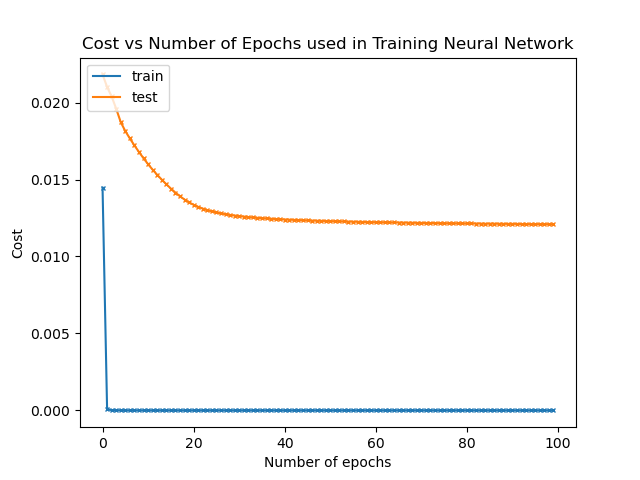
\includegraphics[width=\linewidth]{progress2/figures/cost vs epoch NN.png}
        \caption{Traditional Neural Network}
        \end{subfigure}
        \hfill
        \begin{subfigure}[h]{0.53\linewidth}
        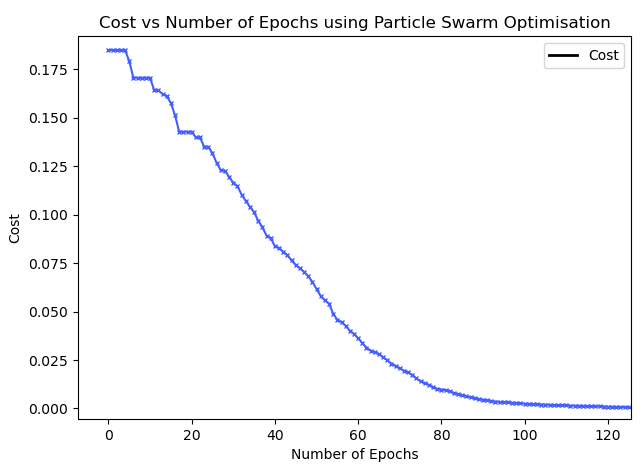
\includegraphics[width=\linewidth]{progress2/figures/cost vs epoch PSO.png}
        \caption{Swarm Optimised Neural Network}
        \end{subfigure}%
        \caption{Graphs showing how the number of epochs impacts the cost function}
    \end{figure}
    
    At small batch sizes the model is more susceptible to noise however similarly with number of epochs, increasing the batch size after a certain point results in no additional gain. It was also found that having a smaller number of more dense hidden layers performed better than creating a larger number of layers.
    
    Fundamentally adjusting these hyperparameters did not result in any significant improvements in accuracy. This was determined to be due to the model detecting local global minima, as a result to the presence of noise in the input data.
    
    \item \textbf{Implementation of Particle Swarm Optimisation}
    
    Upon my supervisor's advice on the local minima problem, I began researching into Particle Swarm Optimisation \autocite{10.1145/3071178.3071208} and its implementation to finding the most optimal hyperparameter values. I was then able to apply this to our current autoencoder achieving better accuracy results than our current neural network configuration as shown in Fig 1.1.1(b). 
    
    One issue is that the python module I decided to use is in a certain format that would require restructuring of our original autoencoder framework which everyone else is using. Despite this issue, we know that this is an approach we can return to, to help in optimising our system in the future. In the meantime I moved to building on our current neural network to aid in global minima detection.
    
    \item \textbf{Investigating Alternative Methods for Global Minima Detection}
    
    To address the global minima detection I have applied convolution layers, drop out layers, and introduced batch normalisation to the current neural network model, which collectively reduce the impact of noise embedded in the data. 
    
    Currently I am also implementing grid search processes to fine tune the hyperparameters however this requires a large amount of computational power so am waiting on my supervisor's request to access university GPU farms. Comparisons with the hyper parameter optimisations from the particle swarm model can then be made. 
\end{itemize}

\subsubsection{Difficulties encountered}

As mentioned before, the problem that arose with our neural network model was that it seemed to get lost in local minima rather than finding the correct global minima via gradient descent. This resulted in undesirable accuracy, around 50\%. Dropout layers and batch normalisation can be used to solve this.

After working on the project for almost a full semester now and having each member having progressed in their own versions of the autoencoder, it is difficult to see how their versions work. Perhaps a longer session over the Christmas break, where each can go through their version in detail will aid in having a better general understanding.
